%% move stuff to defs file

%command inserts todo/comment
\newcommand{\todo}[1]{{\bfseries [[#1]]}}
%% To disable, just uncomment this line
% \renewcommand{\todo}[1]{\relax}

\newcommand{\mrps}[0]{Mref/s}

%\documentclass{acm_proc_article-sp}
\documentclass[10pt,nocopyrightspace,preprint]{sigplanconf}
\usepackage{url}
\usepackage{fancyvrb}
\usepackage{alltt}
\usepackage{graphicx}
\usepackage{comment}
\usepackage[labelfont=bf,font=small,belowskip=-3pt,aboveskip=-5pt]{caption}
\usepackage[compact]{titlesec}
\usepackage{mdwlist}

\begin{document}

%\titlespacing{\section}{0pt}{*0}{*0}
%\titlespacing{\subsection}{0pt}{*0}{*0}
%\titlespacing{\subsubsection}{0pt}{*0}{*0}

%\textheight 9in
%\textwidth 6.5in
%\columnsep 1pc
\renewcommand{\baselinestretch}{0.8}

%\title{Can We Crunch the Social Graph on the Cheap?}
\title{Crunching Large Graphs with Commodity Processors}

%\numberofauthors{7}
%\author{
%Jacob Nelson, Brandon Myers, Andrew Hunter, Dan Grossman, Mark Oskin,
%Carl Ebeling, Luis Ceze\\
%University of Washington\\
%\email{\{nelson, bdmyers, ahh, djg, oskin, ebeling, luisceze\}@cs.washington.edu}\\ \\
%Simon Kahan \\ 
%Pacific Northwest National Lab\\
%\email{skahan@cs.washington.edu}\\ \\
%Preston Briggs\\ 
%Cray Inc.\\
%\email{preston.briggs@gmail.com}\\
%}

\authorinfo{Jacob Nelson$^{\dagger}$, Brandon Myers$^{\dagger}$, A.H. Hunter$^{\dagger}$, Luis
  Ceze$^{\dagger}$,
  Dan Grossman$^{\dagger}$, Mark Oskin$^{\dagger}$, Carl Ebeling$^{\dagger}$, Simon Kahan$^{{\dagger \ddagger}}$, Preston Briggs$^{\dagger}$}{\textdagger University of Washington, \textdaggerdbl Pacific Northwest National Laboratory}{\{nelson, bdmyers, ahh, luisceze, djg, oskin, ebeling, skahan, preston\}@cs.washington.edu}

\maketitle

\begin{abstract}
   Crunching large graphs is the basis of many emerging applications,
   such as social network analysis and bioinformatics. Graph analytics
   algorithms exhibit little locality and therefore present significant
   performance challenges. Hardware multithreading systems (e.g, Cray
   XMT) show that with enough concurrency, we can tolerate long
   latencies. Unfortunately, this solution is not available with
   commodity parts.
 
   Our goal is to develop a latency-tolerant system built out of
   commodity parts and mostly in software. The proposed system includes
   a runtime that supports a large number of lightweight contexts,
   full-bit synchronization and a memory manager that provides a
   high-latency but high-bandwidth global shared memory. This paper
   lays out the vision for our system, and justifies its feasibility
   with a performance analysis of the runtime for latency tolerance.
 
\end{abstract}

\section{Introduction}

Many important emerging applications such as social network analysis,
bioinformatics, and sensor networks rely on crunching very large
graphs. Unfortunately, the computational cost of these applications
gets quickly out of hand. For example, in January 2011, Facebook had
500 million active users with an average of 130 friends each
\cite{Facebook:2011p91}. Its friend suggestion algorithm in 2010 ran on
  a 40-node cluster with 72GB memory per node, and, still, new
  suggestions could only be computed every two days
  \cite{Backstrom:2010p90}. Speeding up these applications at a low
  cost would have a large impact in how we deal with large data-sets and make them even more valuable.

% In January 2011, Facebook had 500 million active users with an average
% of 130 friends each \cite{Facebook:2011p91}.
% Facebook's friend suggestion
% algorithm in 2010 ran on a 40-node cluster with 72GB memory per
% node. Even with that capacity, new suggestions could only be computed
% every two days \cite{Backstrom:2010p90}.


The most interesting computational challenge comes from large,
low-diameter, power law graphs: this combination makes extracting
performance difficult. They do not fit in a single
commodity machine's memory. Their low diameter means that they are
difficult to lay out with locality: every vertex needs to be near every
other vertex. Their power law distribution means that a few vertices
generate much more work than the rest, leading to load
imbalances. Together, these properties \todo{including power law distr?} lead to a
difficult conclusion: each edge traversal is likely to lead to a very
expensive inter-node communication.

Multithreading is a technique that has been used successfully to
implement efficient computations for these graphs. The Cray XMT is an
example of such an approach: it solves the memory latency problem
through concurrency rather than caching. Each XMT processor supports
128 hardware contexts and 1024 outstanding memory operations, and is
able to switch contexts every cycle \cite{tera, feo-xmt}. This ability
comes at a cost: the XMT is an expensive, non-commodity
machine.

\begin{figure*}[htbp]
  \begin{center}
    \vspace{-0.25in}
    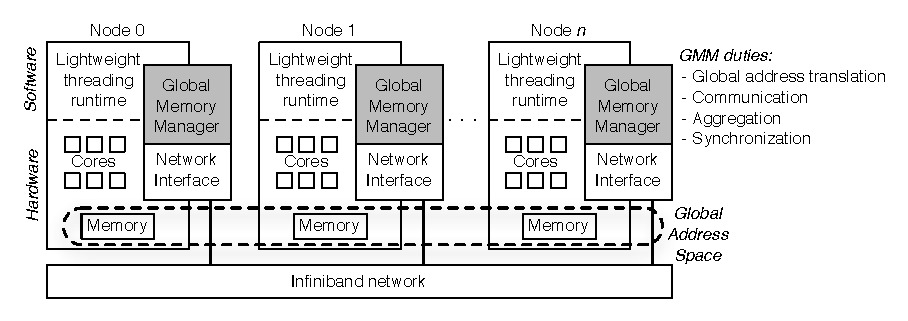
\includegraphics[width=0.7\textwidth]{figures/system-overview.pdf}
    \vspace{-0.1in}
	\end{center}
	\caption{Overview of our proposed system design. The base
          system is a cluster of commodity nodes and interconnect. We
          add a latency-tolerant runtime and a global memory manager
          to obtain efficient access to the global address space. Only
          the shaded components may require hardware design.}
	\label{fig:system-overview}
\end{figure*}


We believe we can build a system based mostly on commodity parts that
can attain XMT-like performance with a familiar, XMT-like,
programming model, but at a fraction of the cost. Therefore, our goal
is to build a system that has good performance on low-locality graph
codes but is implemented with cheap commodity processors and simple
additional support in an FPGA. This approach also has the added
benefit of not sacrificing general-purpose performance.

Figure~\ref{fig:system-overview} shows the structure of our
proposal. It is composed of multiple nodes built with commodity
processors, communicating over an Infiniband network. We add two
components: a runtime system, responsible for executing the user's
threads, and a global memory manager, responsible for facilitating
memory requests to the non-coherent global memory shared across the
nodes.  We are exploring a mix of hardware (FPGA) and software
implementations of the memory manager.
 
This paper describes the vision of our system and explores the
feasibility of our ideas using a single-node implementation of a
lightweight threading runtime. We use prefetch instructions together
with lightweight threads to tolerate the latency of DRAM access on the
local node. We use worst-case pointer chasing benchmarks to
verify our runtime's overhead is acceptable. We also model the effects
of pointer chasing on a remote node by artificially increasing
latencies to several micro-seconds.
 
The rest of the paper is organized as follows. We briefly describe our
programming model in section~\ref{sec:model}. We describe the
implementation of our latency-tolerant runtime and plans for extending
to multiple nodes in section~\ref{sec:approach}. We evaluate our
runtime in section~\ref{sec:evaluation}.  We present related work in
section~\ref{sec:related} and conclude in
section~\ref{sec:conclusion}.


\section{Programming model}
\label{sec:model}

Our goal is to preserve the XMT programming model: large shared global
address space, explicit concurrency with a large number of threads,
and full-bit synchronization.  We partition the overall address
space into a global shared address space and per node private address
spaces. Locality may be exploited directly by the programmer in the
node private address spaces, just as in a conventional cache-coherent
multiprocessor node. In contrast, locality cannot be exploited in the
global space: its value is in providing high bandwidth random access
to any word in a shared data structure by any processor.

% Whereas in the PGAS model coherency of global copies is implicitly
% maintained across the system, % \todo{cite pgas?}
% we completely forego
% caching of globally shared data.  

% A node can exploit temporal locality of data stored in the global
% space only by first copying it into the node's local space.  In this
% way, a node can access data at random across the system while
% incurring no hardware coherence overhead: consistency is enforced by
% our mechanisms for explicit global synchronization.

The model promises efficiency subject to the presence of sufficient
concurrency.  Exactly how that concurrency is expressed by the
programmer is language dependent. The goal of our system is to support
that concurrency and consequently provide latency tolerance on a large
address space. We do so via software multithreading: computation that
is about to execute a long latency operation (e.g. a remote memory
reference) initiates the operation and then yields to the scheduler,
which quickly resumes execution of another computation.  Concurrency
is also used\todo{vague}---via aggregation of requests to a common node
destination---to make more efficient use of network bandwidth and in
some cases reduce bandwidth demands.

Synchronization on locations in the node private address space is the
same as on conventional systems.  Synchronization on global addresses
works differently: we provide atomic operations such as {\tt
  int\_fetch\_add} as well as operations using full-bits, as on
the Cray XMT.  As is true for other long latency operations,
synchronization latency is tolerated by yielding to the scheduler.
Even non-blocking global atomics yield so the core can switch to
another computation while the synchronization is accomplished outside
of the pipeline.  In addition, the implementation can exploit
aggregation when concurrency is abundant to increase the throughput of
global synchronization.

\section{Implementation}
\label{sec:approach}
Our goal is to use multithreading to tolerate
the latency of random accesses to memory in a global address space
spread across multiple nodes.  Our implementation must provide three features:
\begin{description}
\item[Lightweight multithreading:] We expect to need hundreds of
  threads to tolerate a cluster's network latency, so our threading
  implementation must have low overhead.

\item[Concurrency in global memory references:] A thread making a
  long-latency global memory reference must be able to yield and allow
  other threads to make progress.

\item[Low overhead synchronization:] 
%  We must support global synchronization between threads that allows unrelated threads to proceed unblocked.
  A thread that is synchronizing must yield its core to allow others to make progress. \todo{repetitive with the previous item}
\end{description}
We discuss our approach to solving each of these challenges in
turn. For each one, we discuss both our current single-node
implementation and ideas for a multi-node implementation.

\subsection{Lightweight multithreading}

Our approach to supporting many lightweight threads uses a
cooperative, user-level multitasking system built using
coroutines. Much work has been done on similar user-level systems
\cite{ult,capriccio}, but we have more stringent requirements:
coroutines must use little space so that many can be active without
trashing the cache; and context switches must be fast (a small
fraction of memory latency) so that we can overlap memory requests and
achieve concurrency.

%We minimize context size by treating context switches as function
%calls, as in~\cite{charm}. This allows us 
%to save and restore the
%minimum number of registers allowed by the ABI, and 
%Simon:  not really true -- we could save fewer if we knew which of the
%callee save registers weren't going to be clobbered.
\todo{decide whether to change these 2 paragraphs to be inclusive of other lightweight implementations, like jump table}
We treat context switches as function calls, as in~\cite{charm}. This allows us 
to depend on the compiler to save and restore caller-save registers while we explicitly save and restore all the callee-save registers.  We minimize
context switch time by doing all switching and scheduling in user space.

%\paragraph{Single-node implementation.}  
In our single-node implementation, we implemented coroutines
as described, with a round-robin scheduler. Coroutines do local work,
issue a remote prefetch, and switch to the next in turn.  When the
coroutine is reactivated, it assumes the requested data is available
and issues a read.  If the data is not yet received and in cache, the core
(and all its coroutines) can stall.

%\paragraph{Multi-node ideas.}
As we develop our multi-node implementation, we will explore how the memory manager and coroutine scheduler may
interact, so that threads waiting on long-latency memory operations or
synchronization operations will be scheduled soon after their
operations have completed.

\subsection{Concurrency in global memory references}

To enable concurrency in memory references, we break each read or
write into two operations: the {\em issue} operation and the {\em
  complete} operation. The read issue operation starts data moving
towards the processor and returns immediately, like a prefetch; the
read complete operation blocks until data is available. The write
issue operation takes data along with an address, and starts an
asynchronous write; the write complete operation blocks until the
write is committed.

A read operation in user code consists of three steps: a {\em read
  issue}, which causes the data to start moving; a {\em yield}, which
causes another thread to start executing, overlapping the read
latency; and, once the reading thread has been rescheduled, a {\em
  read complete} blocks until the data is available. A write operation
follows the same pattern.

%\paragraph{Single-node implementation.}
In our single-node implementation, we use prefetch instructions for the issue operation, and regular
blocking reads and writes for the complete operation.  Since we expect
these global references to have low locality, we use the
``non-temporal'' form of prefetch to avoid disturbing the state of the
cache hierarchy \cite{intel:swdev}.

%\paragraph{Multi-node ideas.}
As we develop our multi-node implementation, we believe we will need hundreds of outstanding memory references per
processor to cover the latency of remote references in a multi-node
system. Unfortunately, commodity processors have much smaller limits
on memory concurrency: section~\ref{subsubsec:evalsinglebase} finds a
limit of 36 concurrent loads. We will have to manage memory
concurrency on our own to avoid this limit. We describe approaches in
both software and hardware.

One approach is for user code to delegate global references to a
special {\em global memory manager thread}, running on another core in
the chip. This thread translates the global address into a network
destination, makes the request through the network card to the remote
node, checks for completion, and delivers the returned data to the
requesting thread. On the remote node, the remote memory manager
thread would perform the memory operation and return the data to the
requesting node.

%This approach has the benefit of enabling our entire system to be
%build using commodity parts, but its potential for performance is not
%clear. We have increased the overhead of a single memory operation:
%what in the single node case was a simple read, is now multiple
%queuing operations between threads and multiple reads and writes over
%the processor's link to the network interface.

Another approach moves the global memory management to a hardware
device. We can add a coprocessor FPGA in a processor socket, listening
to coherence messages on the bus, similar to \cite{mogill}. Note that
this accelerator is only a memory proxy, not a compute
coprocessor. The accelerator would map all global shared memory into a
segment of each node's local address space; when it detects a
reference to memory on a remote node, it would do the address-to-node
translation and issue the request through the network controller,
delivering the data to the requesting thread when ready. We would
encode commands in the upper bits of the address; a read from a
location's {\em issue} address start the remote request and return
immediately, and a read from a location's {\em complete} address would
block until the data was available.


%To support the issue and complete operations for concurrency support,
%commands would be encoded in the upper bits of the address: then each
%remote word would have multiple addresses on the local node. Reading
%from the {\em issue} address would immediately return a value
%indicating that the accelerator is issuing the request over the
%network. Reading from the {\em complete} address would block until the
%data was available.

With either approach, the question of request aggregation will be
important. Each memory request we make is small: 8 bytes is a likely
size. But most networks are optimized for bulk transfers of a few
thousand bytes. To improve network utilization, we will explore the
aggregation of multiple memory operations to different addresses on
the same remote node. 


\subsection{Low-overhead synchronization}

Just as with reads and writes, we enable concurrency around
synchronization operations by splitting them into {\em issue} and {\em
  complete} phases.

Implementing full-bit support efficiently on a platform not
designed for them is a challenge. Previous work \cite{qthreads} has
enabled support for full-bit synchronization on arbitrary words by
allocating additional storage for the full-bits and implementing
atomic full-bit operations as library routines.

One potential optimization is to limit full-bit synchronization to
pointers to aligned data types, and reuse wasted space in the
low-order bits of the pointer for full-bit storage. These bits
would be masked out when the pointer is returned to the user.  This
allows us to synchronize any data type through one level of
indirection.

%\paragraph{Single-node system.}
In our single-node implementation, we prefetch and yield before performing
a synchronization operation. We support only the synchronization
operations supported by our development platform; we have not
implemented full-bits yet.

%\paragraph{Multi-node ideas.}
In a multi-node implementation, synchronization operations can be delegated to a memory manager
thread or accelerator. Synchronization on remote data would be
performed by the remote memory manager. This may simplify the
implementation: if only a single core (or single accelerator) is
accessing the data being synchronized, the use of memory fences may be
reduced or eliminated.

% 2TB global memory => 68GB of distributed FE bits.  This seems reasonable, given that a 2TB system might have 64 nodes, so ~1GB per memory manager if one manager per node.

\section{Evaluation}
\label{sec:evaluation}

Our goal is to evaluate the feasibility of our proposed runtime. We
want to determine two things: whether coroutines can generate memory
concurrency while incurring minimal performance overhead, and whether the system can support the level of concurrency required to tolerate the latency that will be present in a multi-node system.

We focus the evaluation on one component of the runtime: lightweight context switching. We ran pointer-chasing benchmarks on a single-node implementation of our runtime. These pointer chasing experiments are intended to model a particular ``worst-case'' behavior of irregular applications, where each memory reference causes a cache miss.

We ran these experiments on a Dell PowerEdge R410 with two Xeon X5650 (Nehalem microarchitecture)
chips and 24GB of RAM, with hyperthreading disabled. These
chips use a NUMA memory architecture, where each chip has
its own integrated memory controller and DIMMs; references to other
chips' memory are carried over Intel's cache-coherent QuickPath
Interconnect (QPI) \cite{quickpath:website}.

Our evaluation consists of two parts. First, we demonstrate that the
runtime system can achieve the same performance as when 
explicit memory concurrency is available. Second, we look at the runtime
within the multi-node picture and show that it can tolerate large
latencies. In each part we begin by studying relevant aspects of our
test machine's memory system so we can interpret our runtime results.


\subsection{Single-node performance}

% We first characterize the performance of our test machine's memory
% system. Then we use these results to evaluate the performance of our runtime within a single node.

\subsubsection{Base memory system performance}
\label{subsubsec:evalsinglebase}

We measured two parameters: the maximum random reference
rate that can be issued by the cores in one chip and the maximum random
reference rate that can be serviced by one chip's memory controller. 

To find the maximum random reference rate that one chip's cores
can issue, we ran pointer chasing code following the model of
Figure~\ref{fig:code}a. Each core issues $n$ list traversals
in a loop; we call $n * \textit{number of cores}$ the number of
{\em concurrent offered references}, since the memory system may not
be able to satisfy them all in parallel. Since our goal is to find a
baseline for evaluating our coroutine library, we depend on the
cores' exploitation of ILP for memory concurrency, rather than our coroutine
library.

\begin{figure*}[ht]
\vspace{-0.2in}
%list walk ILP
\begin{minipage}[b]{0.3\linewidth}{\small
\centering
\begin{alltt}{\scriptsize
  while (count-- > 0) \{
    list1 = list1->next;
    list2 = list2->next;
    \ldots
    list\(n\) = list\(n\)->next;
  \}
  }\centering{\bf (a)}
\end{alltt}
%\caption{Pseudocode for pointer chasing without coroutines.}
\label{fig:pointernocoro}
}\end{minipage}
%listwalk green threads
\begin{minipage}[b]{0.35\linewidth}{\small
\centering
\begin{alltt}{\scriptsize
  while (count-- > 0) \{
     prefetch(&(list1->next));
     switch();
     list1 = read(&(list1->next));
 \}
 }\centering{\bf (b)}
\end{alltt}
  %%n lists
  % while (count-- > 0) \{
  % prefetch(&(list1->next));
  %   prefetch(&(list2->next));
   %  \ldots
   %  prefetch(&(list\(n\)->next));
   %  switch();
   %  list1 = read(&(list1->next));
   %  list2 = read(&(list2->next));
   %  \ldots
   %  list\(n\) = read(&(list\(n\)->next));
%\caption{Pseudocode for pointer chasing using coroutines.}
\label{fig:pointercoro}
}\end{minipage}
%cache pressure
\begin{minipage}[b]{0.32\linewidth}{\small
\centering
\begin{alltt}{\scriptsize
  while (count-- > 0) \{
    prefetch(&(list1->next));
    switch();
    list1 = read(&(list1->next));
    for( i in 1 to num_local_updates ) \{
      local->data++;
      local = local->next;
   \} \}
   }\centering{\bf (c)}
\end{alltt}
%\caption{Pseudocode for pointer chasing with local updates.}
\label{fig:pointerupdate}
}\end{minipage}
%\vspace{5pt}
\caption{Pseudocode for: (a) pointer chasing without coroutines, (b) pointer chasing using coroutines, (c) pointer chasing with local updates. Coroutine code, as in (b), might also include ILP like what (a) depends on for memory concurrency, e.g., by doing multiple prefetches to independent lists, switch, then multiple reads.}
\label{fig:code}
\end{figure*}

The lists were laid out randomly with pointers spaced at a cache line granularity, maximizing
the probability of each reference being a miss. We allocated the lists
on 1GB huge pages to minimize TLB refill overhead.

\begin{figure}[t]
  \vspace{-.1in}
	\begin{center}
		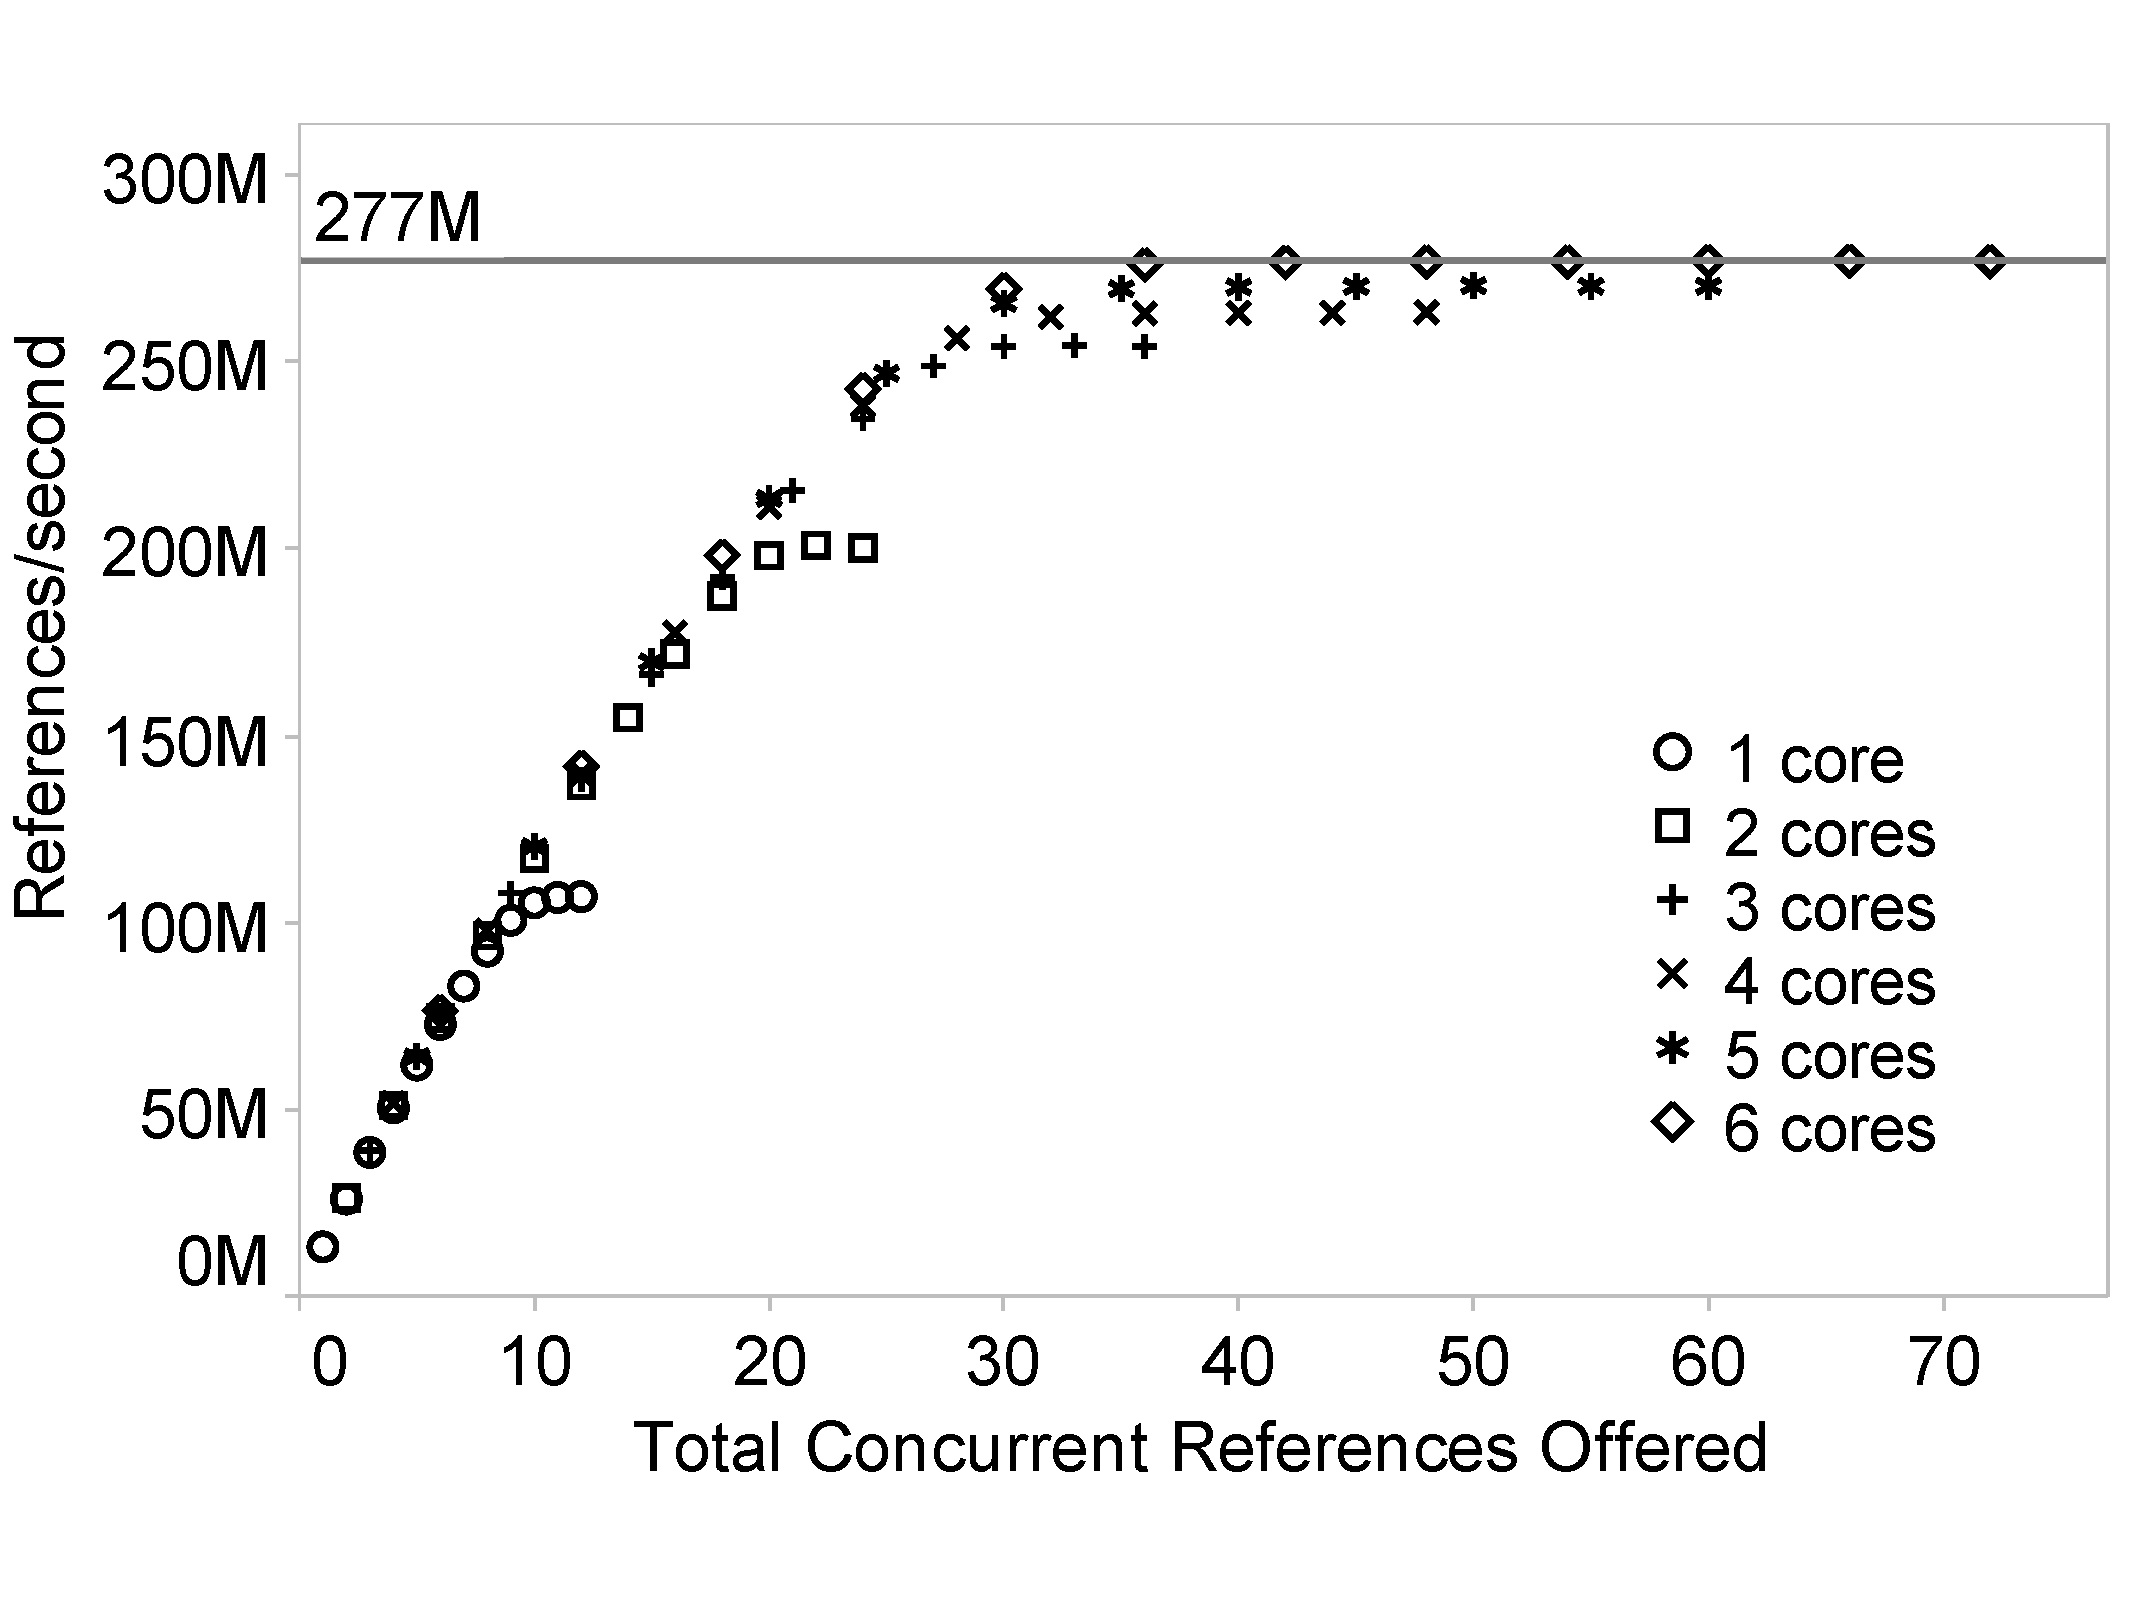
\includegraphics[width=0.47\textwidth]{figures/multi-listwalk-totalconc-edited.pdf}
	\end{center}
	\caption{Throughput of listwalk versus total number of
          concurrent references offered by the cores. Data points for
          running 1 core are shown as circles, and data points for
          running 6 cores are shown as diamonds. 
%Notice that the throughput for a single core levels out at 10
%concurrent references. For 4 to 6 cores, the throughput levels off at
%around 36 references, which seems to be the most memory concurrency a
%processor can handle.
        }
	\label{fig:listwalk-totalconc}
\end{figure}

Figure~\ref{fig:listwalk-totalconc} shows the result. Each point represents
the maximum rate pointers are traversed for a given number of
concurrent offered references. We see a maximum rate of 277 million references per second (\mrps), which agrees with the measurements found by \cite{Mandal:2010}. This rate is achieved when the number of offered references is 36. Note that a single core cannot support this level of
memory concurrency; the maximum reference rate for a single core is
107M. We believe this limit is due to the core having only enough {\em line fill
  buffers} \cite{nehalem:arch} to store 10 concurrent private cache misses.

The memory controller in the chip has more bandwidth than its
cores can saturate. To measure the memory controller's maximum random
reference rate, we extended the previous experiment so that cores in
both processors were traversing lists allocated in the first processor's
memory. With this configuration, we observed a maximum rate of 360
\mrps. We believe this difference is due to the chip having only 32 buffers in its {\em Global Queue} \cite{nehalem:perf} for tracking concurrently-executing read misses from all the cores' private caches.


\subsubsection{Coroutine performance}

To evaluate the performance of our runtime, we investigated two
effects: the maximum reference rate using coroutines
to obtain memory concurrency and the effects of cache pressure from the
coroutines' context storage. 

To find the maximum reference rate obtainable using our coroutine
library, we modified our pointer chasing benchmark as shown in
Figure~\ref{fig:code}b. Recall that the baseline code in Figure~\ref{fig:code}a relied solely on ILP to achieve memory concurrency, which may not be abundant in real applications. Using coroutines, there are two sources of offered
concurrent references: the ILP exploited by the processor, and the
memory concurrency enabled by prefetching and switching to a new
coroutine. As with our first experiment, we allocated the lists in the
same processor as the cores doing the traversal. 

\begin{figure}[t]
  \begin{center}
    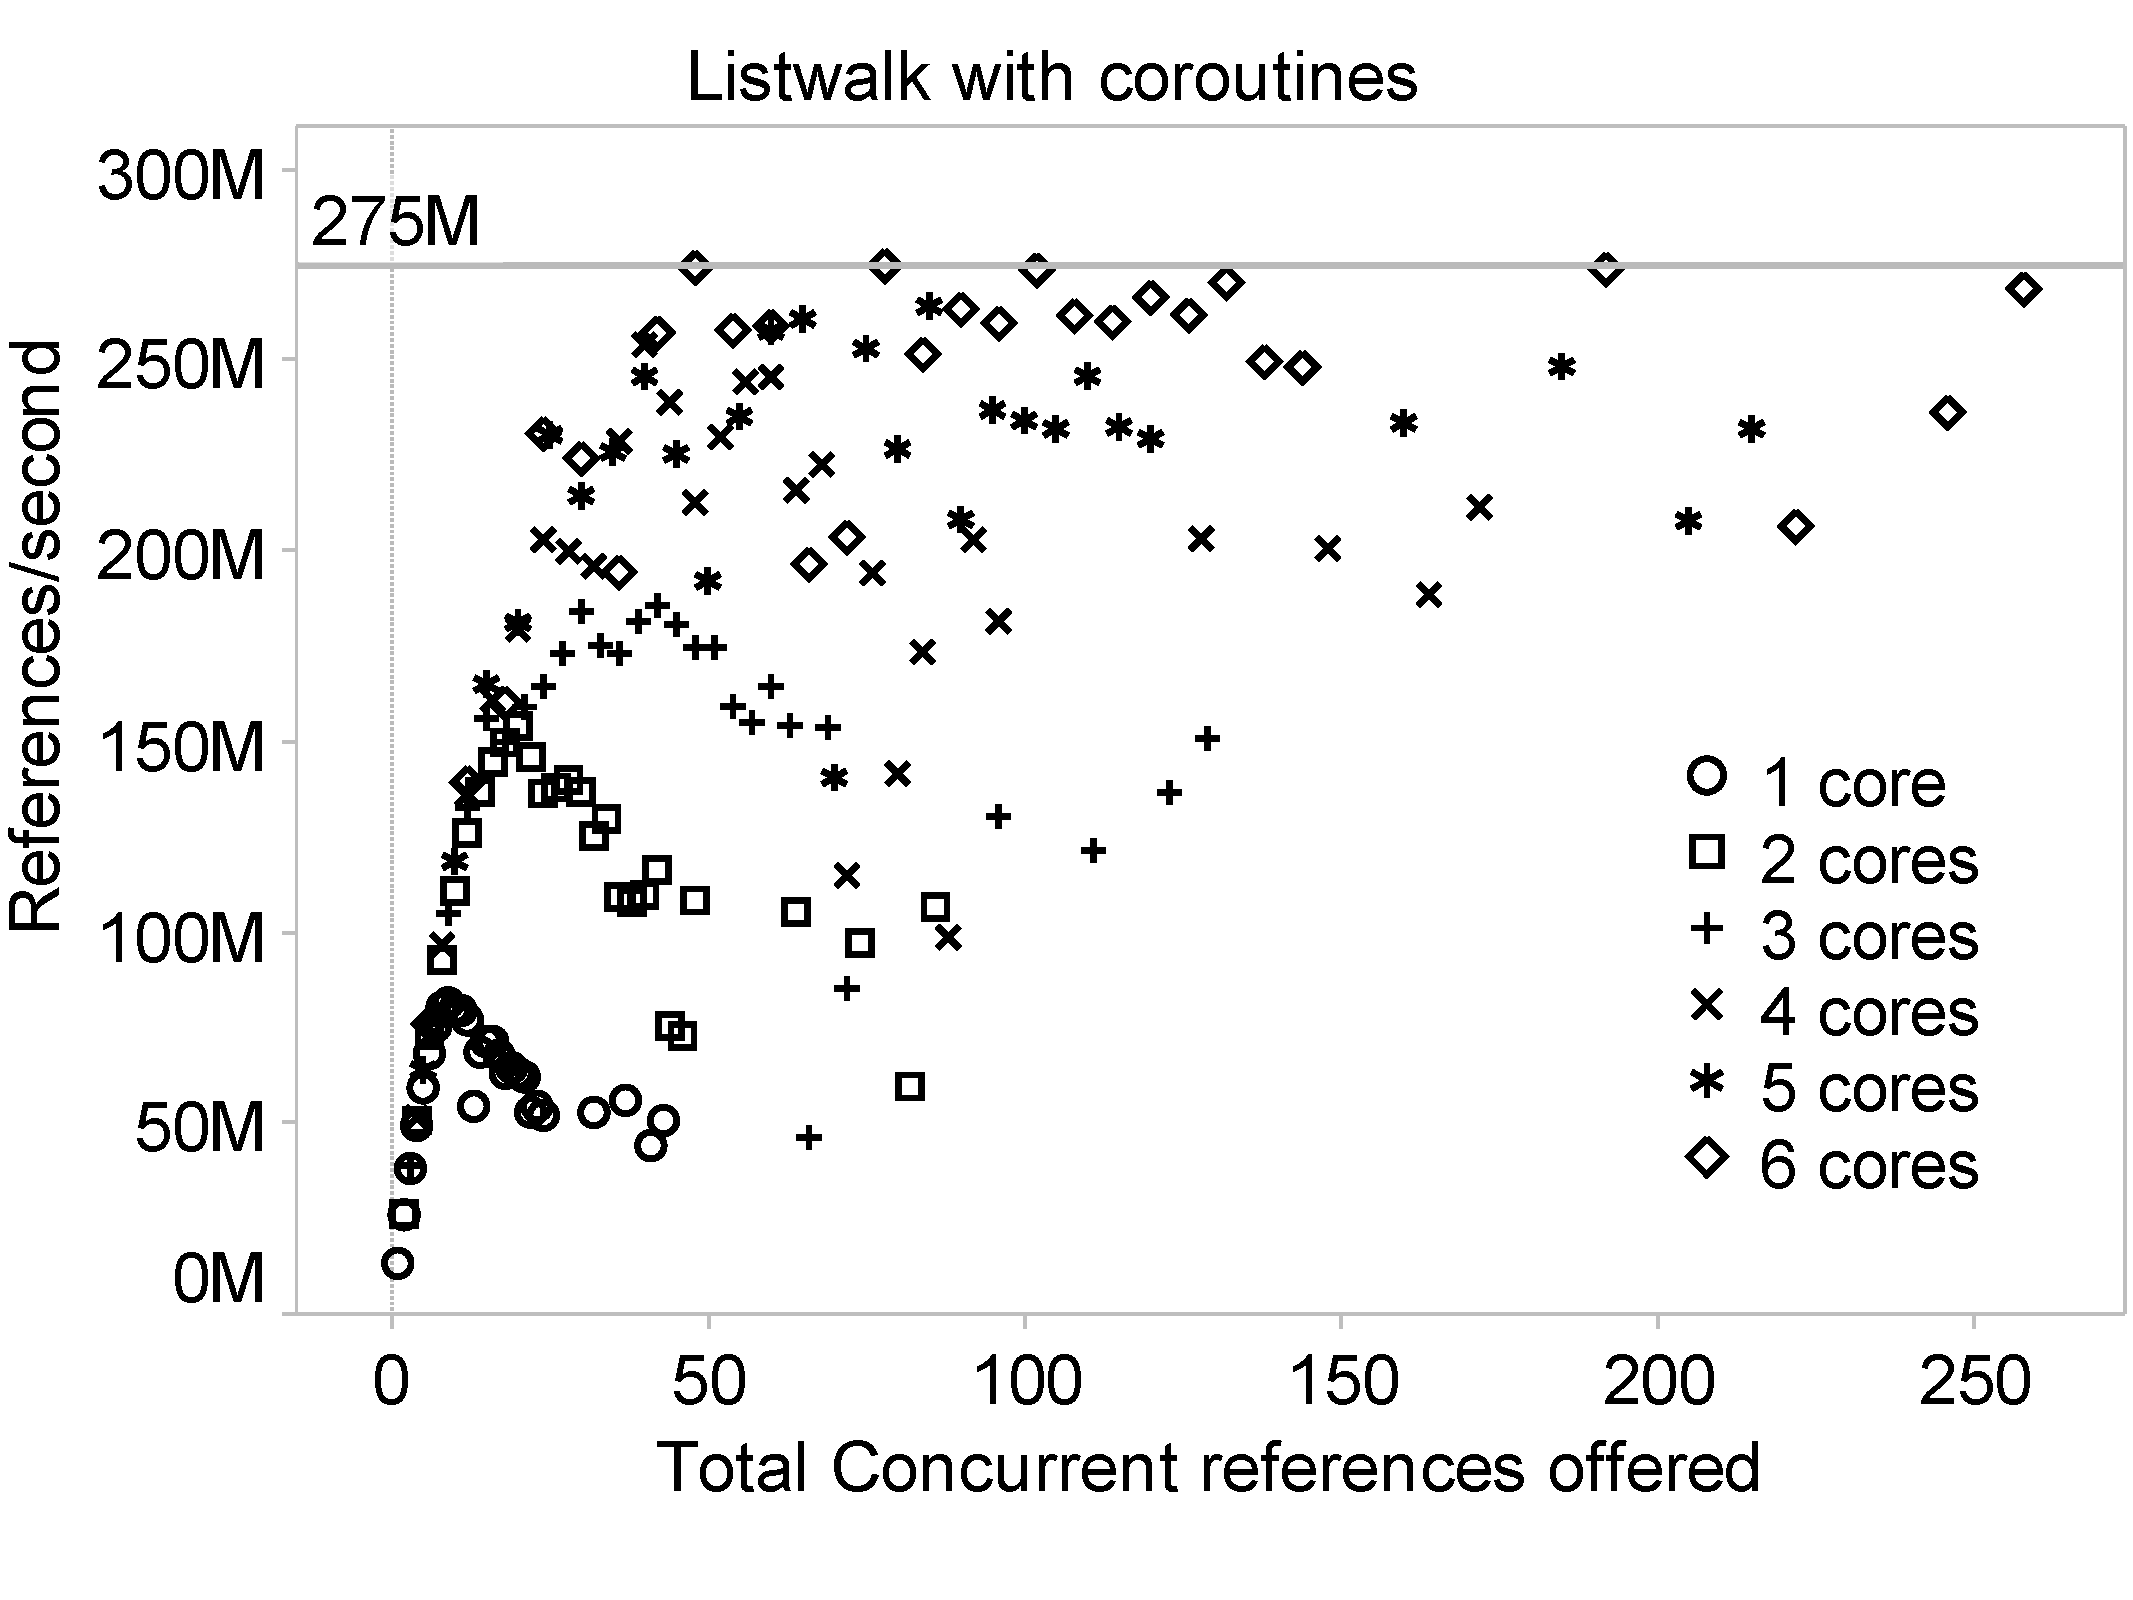
\includegraphics[width=0.47\textwidth]{figures/multi-green-edited.pdf}
  \end{center}
  \caption{Pointer chasing with coroutines, with one reference per
    coroutine. Number of coroutines per core is $\textit{total concurrent references} / \textit{number of cores}$.}
  \label{fig:multi-green}
\end{figure}

Figure~\ref{fig:multi-green} shows the result. For this
experiment, we limited memory concurrency to one concurrent miss per
coroutine, so the only source of memory concurrency is the use of
coroutines. We are able to obtain a rate of 275 \mrps\ with 48 concurrent misses, or 8 coroutines per core. These
results are very close to the ILP-only experiment, but more concurrent requests are required--about 48 versus 36. When the number of references per coroutine is larger than 1, fewer coroutines are required to reach full performance.

We observe a gradual decrease in reference rate once the number of
concurrent references per core exceeds 10; we believe this is due to
later prefetches squashing earlier ones in the line fill buffers. In the real runtime we expect this effect will not exist, since prefetch will not be implemented with built-in non-temporal prefetch instructions. We
also observe many points that do not follow the trend are below the max, and these results are repeatable. This effect is harder to explain, but we suspect it is
due to resource contention in the cores' pipelines once the memory
system is full of requests. 

%Such points are repeatably lower, and looks like the std dev of such points (the diamond ones than are low) is also higher than other "normal" points: around 35M versus 13M or less, which seems to suggest a weird effect at those numbers}


The stacks for the coroutines are stored in the data cache, where they
will compete for space with an application's data. To characterize the
effects of this cache pressure, we modified our list chasing benchmark
to include random updates to a per-coroutine local data structure that
is small enough to fit in cache. Figure~\ref{fig:code}c shows the
general idea.

% cache pressure figure
\begin{figure}[h]
  \begin{center}
    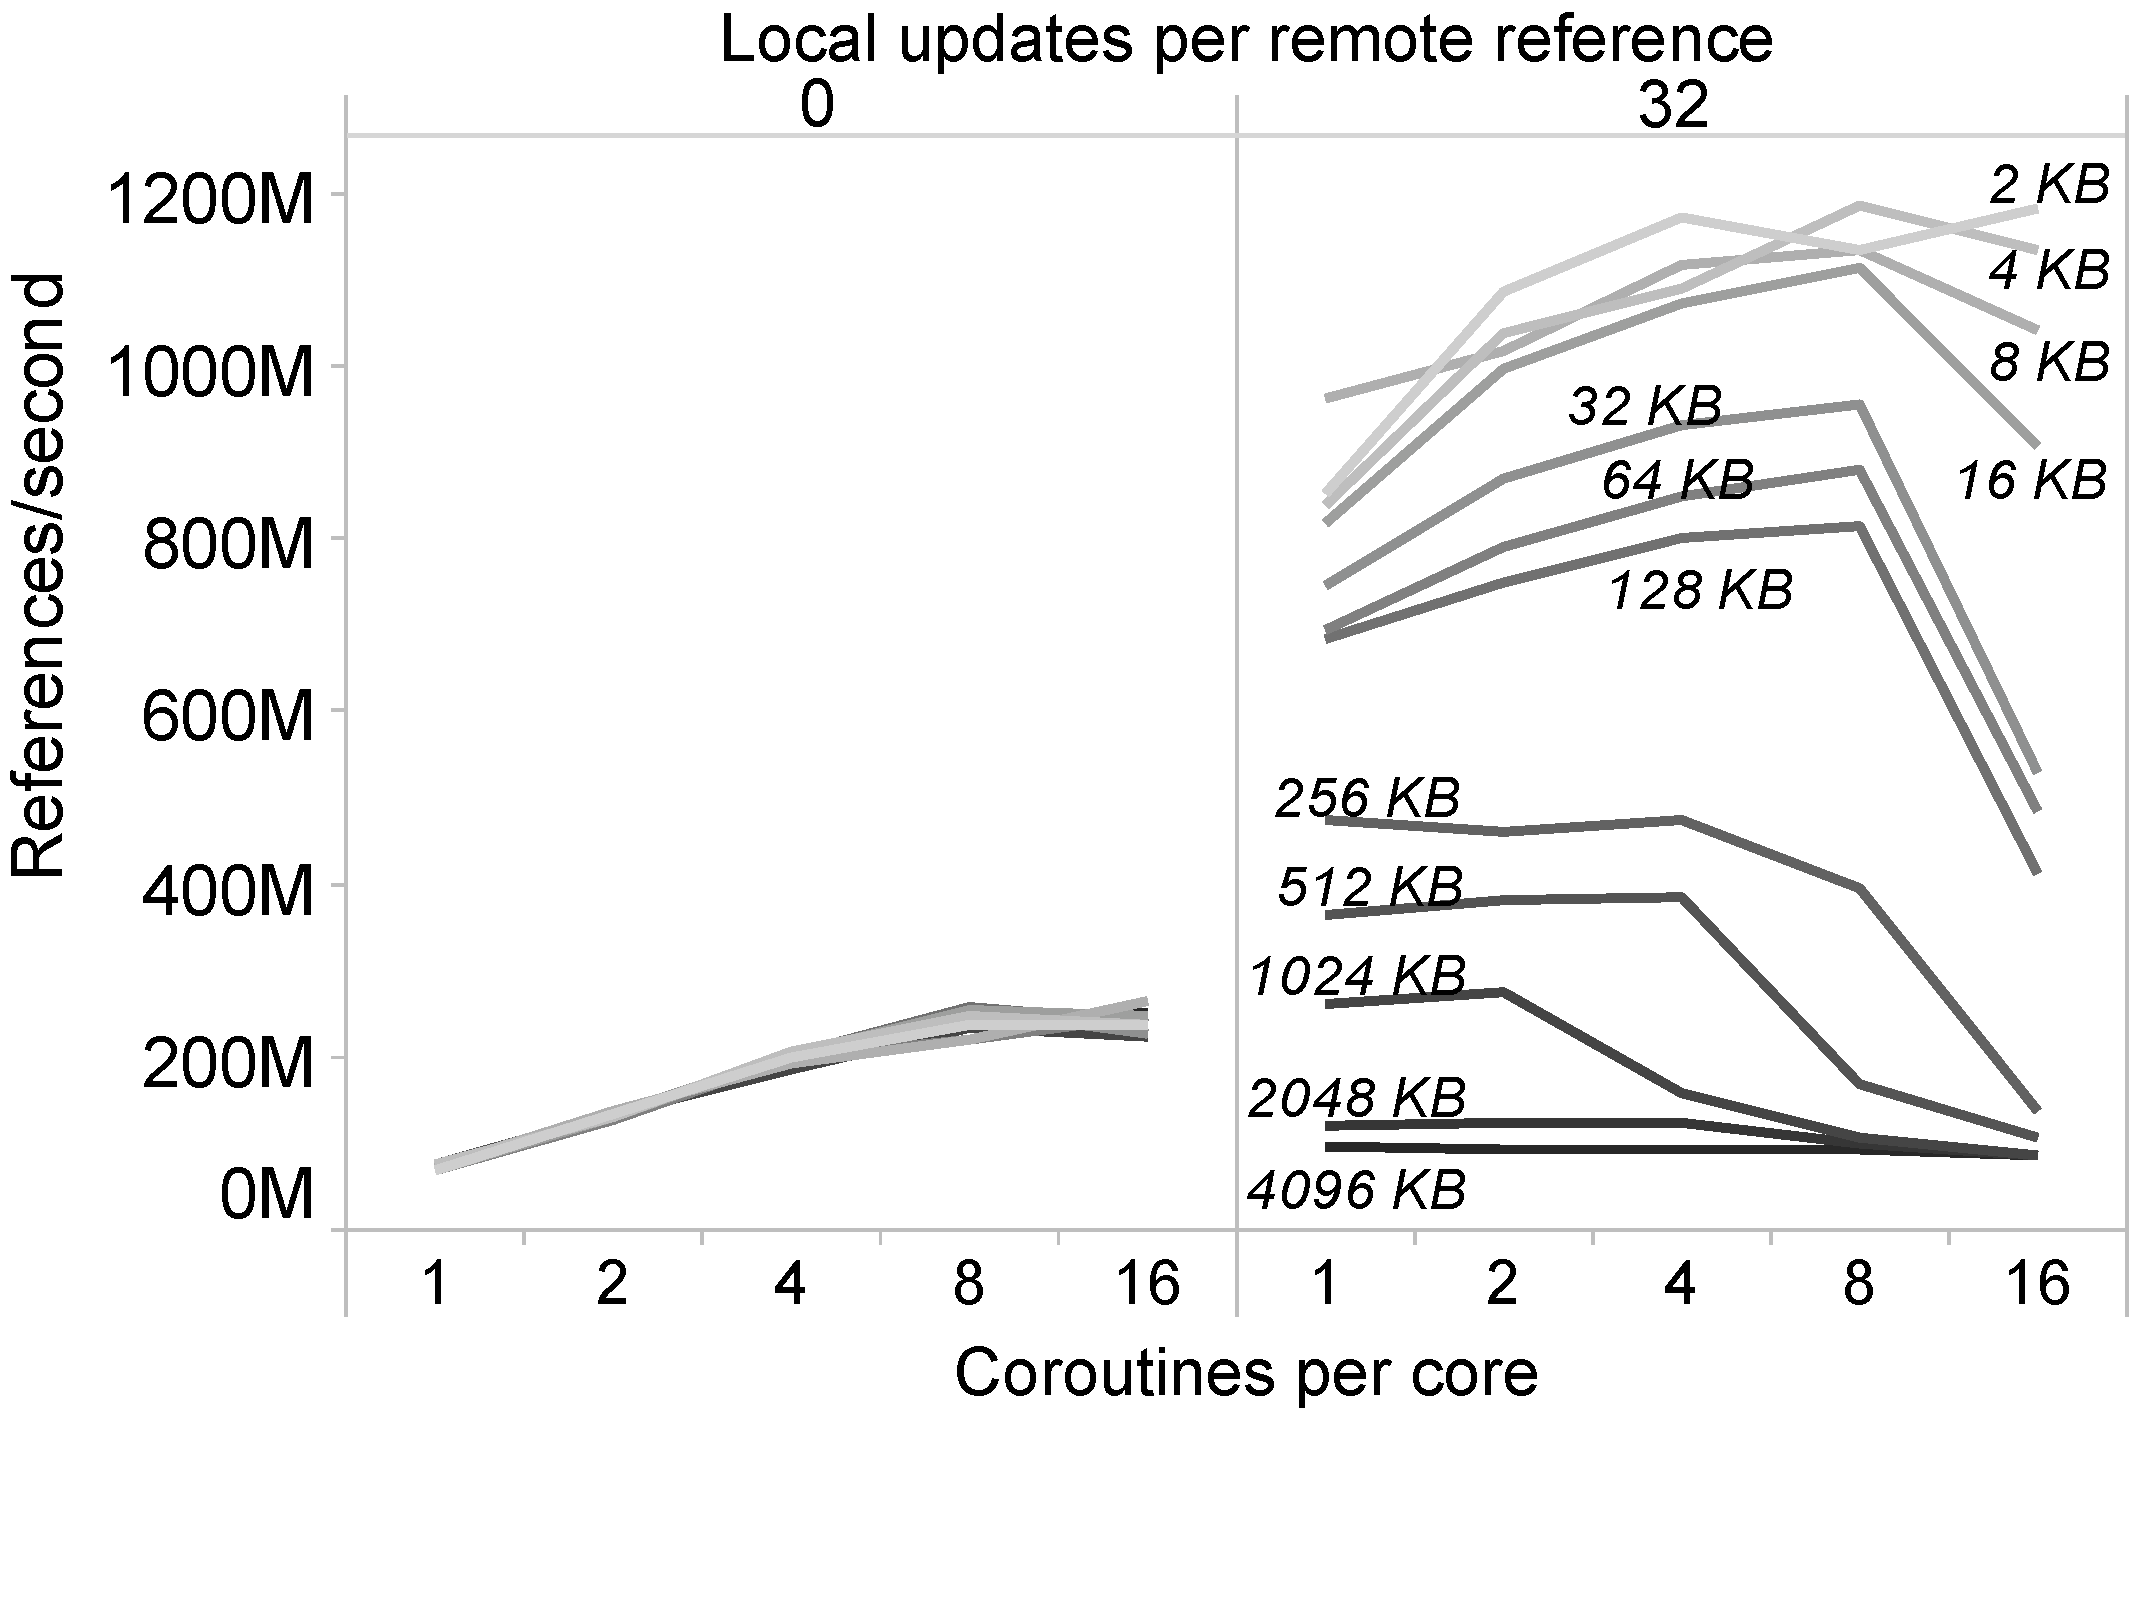
\includegraphics[width=0.42\textwidth]{figures/cache-pressure-edited.pdf}
  \end{center}
  \vspace{-0.3in}
  \caption{Cache pressure with coroutines, on six cores.}
  \label{fig:cache-pressure}
\end{figure}

We varied the size of the local working set from 2KB
to 4MB, and ran both 0 and 32 local updates for each pointer
traversal. We measured the overall reference rate, including both the local updates and remote references.

Figure~\ref{fig:cache-pressure} shows the result. As we would expect,
when there are no references to the local structures, the reference rates grow with the number of coroutines just as in
Figure~\ref{fig:multi-green}. For 32 local updates per traversal, while performance
decreases for large working set sizes and large numbers of coroutines,
we see speedup as the number of coroutines increases up to 128KB working set size with 8 coroutines per
core. \todo{preempt questions about drop at 16 which is much less than the about 50 needed per core by saying that the drop is likely the same drop effect seen earlier, which is likely to be prefetch squashing since it happens at number of line fill buffers}

\subsection{Performance with multiple nodes}

To evaluate the potential for our runtime to perform in the multi-node case, we simulated a network delay and saw whether the runtime could tolerate the larger latency. 

Since the network interface is accessed over QPI, we estimated QPI bandwidth by measuring the QPI communication between the two chips of our test machine. To do this, we allocated the lists in the second chip's memory and ran the traversals on the first chip's cores. We found that use of the QPI link limits us to 175 \mrps.

% take this figure out if we need the space
% maybe even take out whole QPI thing and just relate the 100M?
% the main point is room for remote references to local memory
%\begin{figure}[h]
 % \begin{center}
  %  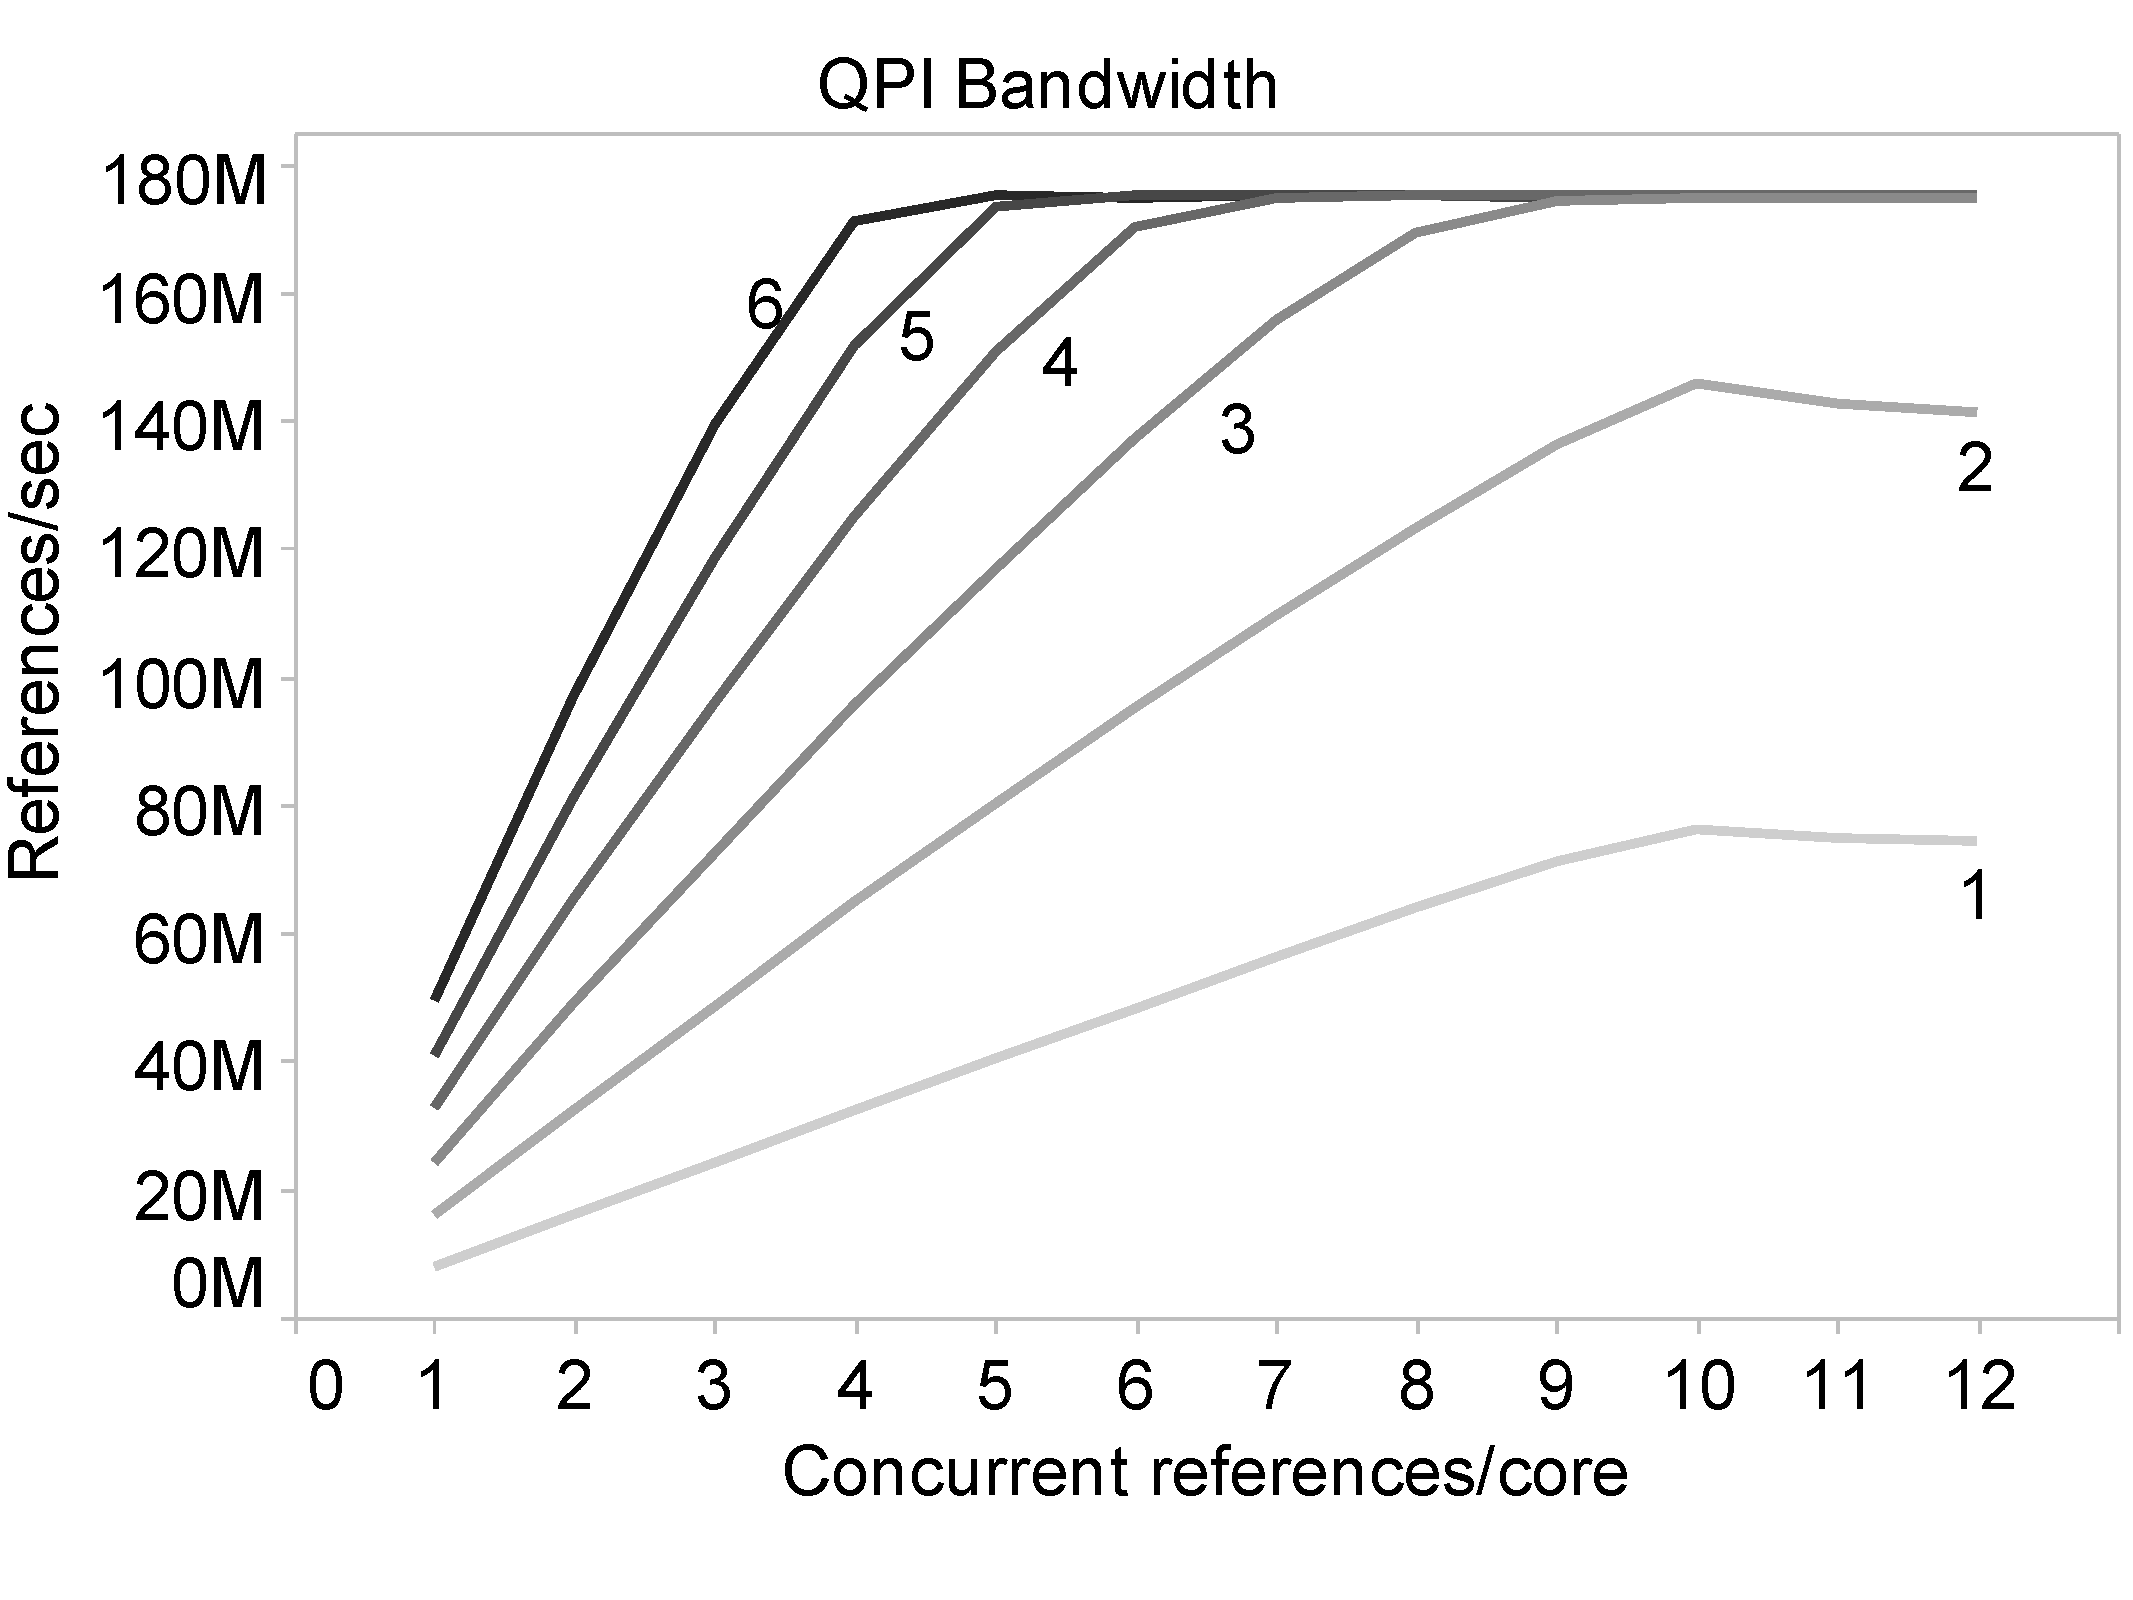
\includegraphics[width=0.42\textwidth]{figures/qpi_bw-edited.pdf}
 % \end{center}
 % \caption{Pointer chasing in a remote processor's memory.}
 % \label{fig:listwalk-qpi}
%\end{figure}
%%%%%%%%%%

To simulate the performance of pointer chasing in a multi-node system,
we modified the scheduler of our coroutine library to include a delay
before a coroutine can be rescheduled, imitating the network transit
delay even though we are referencing local memory. We assume 1.1
$\mu$s interface and 400 ns switch latencies in each direction
\cite{infiniband, mellanox:site}, and thus estimate a 3 $\mu$s round-trip
delay.

%simulated delay plot
\begin{figure}[h]
  \begin{center}
    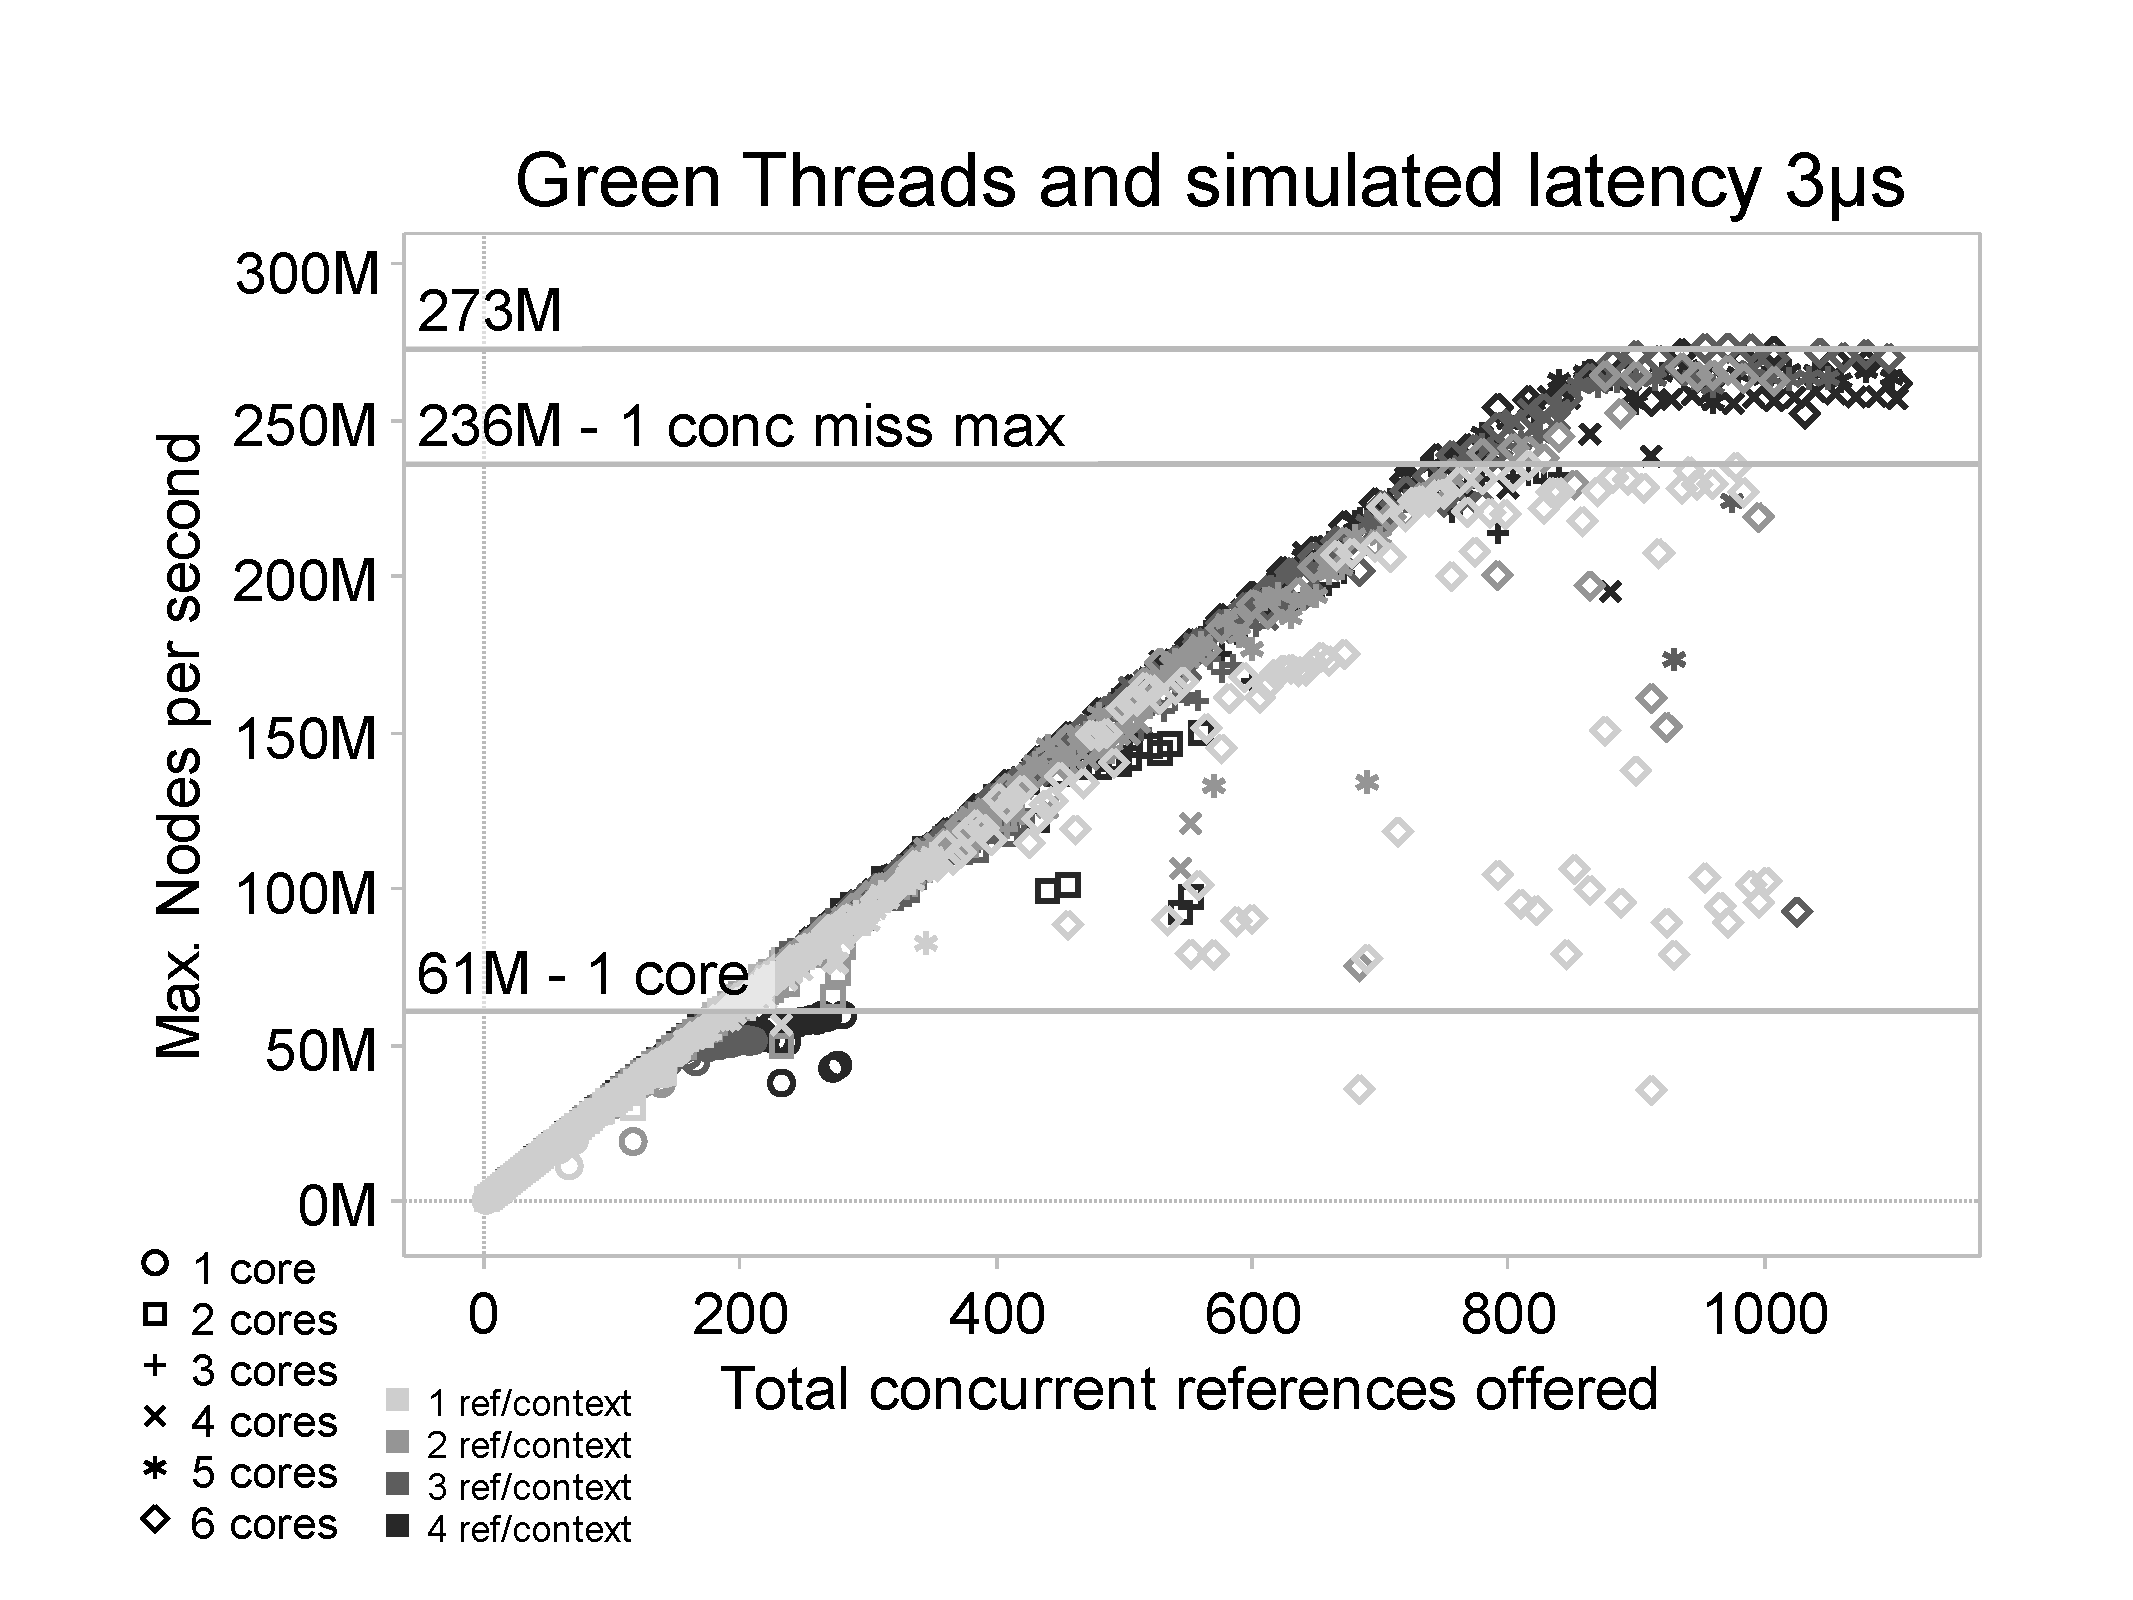
\includegraphics[width=0.47\textwidth]{figures/multi-green-delay7800-edited.pdf}
  \end{center}
  \vspace{-0.3in}
  \caption{Pointer chasing with simulated network delay. Each core ran up to 167 coroutines, and each coroutine made 1 to 4 concurrent references.}
  \label{fig:network-delay}
\end{figure}

The results of the experiment are shown in
Figure~\ref{fig:network-delay}. We are still able to reach a
near-maximum rate of 273 \mrps\footnote{The throughput keeps increasing up to around 850 total concurrent references offered, far more than the 36 we know the chip to support. This is because we have modeled the network latency by forcing coroutines to wait the extra time before using the data, so the physical miss buffers on our machine are not tied up any longer than usual.}, but at least 2
concurrent references per coroutine are required. Running with one
reference per coroutine achieves 236 \mrps. 

These results suggest that the runtime should be able to tolerate
large latency well enough to exceed the max issue rates of both modern
network interfaces (about 100 \mrps) \cite{mellanox:press} and the QPI
link used to reach the network interface.

%Any network interface would be connected through a QPI link,
%which we measured to have a bandwidth limit of 175 \mrps, so our runtime appears to have the capacity to chase pointers
%in a remote memory. 

\todo{also have results that remote cores over QPI plus delay 3us can make it up to the 175M, with sufficient number of coroutines}


\section{Related work}
\label{sec:related}


Much work exists on using multithreading to tolerate latency. Hardware
implementations include the Tera MTA~\cite{tera} and Cray
XMT~\cite{feo-xmt}, Simultaneous Multithreading \cite{tullsen-smt},
MIT Alewife \cite{agarwal-alewife}, Cyclops \cite{almasi-cyclops}, and
even GPUs \cite{gpus}. Software-only approaches exist as well; the
Software Controlled Multithreading project \cite{mowry-scm}, QThreads
\cite{qthreads}, MAESTRO \cite{maestro}, and Charm \cite{charm} all
use variants of this idea.
%In contrast to all of these, our goal is to tolerate
%latencies across a multi-node system using mostly software.

There has also been much work on user level threading, including the First-Class
User Level Threading project \cite{ult} and Capriccio \cite{capriccio}. We have a
different goal; we want many lightweight contexts to tolerate memory
latency.

Our goal of presenting a global view of distributed memory to the
programmer is shared by the PGAS community, and is used in languages
like Chapel \cite{chapel}, X10 \cite{X10}, and UPC \cite{upc}. They
obtain performance by minimizing references to remote nodes, whereas we
design for remote references.

The idea of processing large graphs on distributed machines has been
explored by projects such as Pregel \cite{pregel}, the Parallel Boost
Graph Library \cite{parallelbgl}, and CGMLib \cite{cgmlib}. Our goal
is to develop infrastructure to aid implementation of similar
libraries.

\section{Conclusion}
\label{sec:conclusion}

We presented our plans for building a system for large graph
computation using commodity parts. We leverage decades-old ideas on
using a large amount of concurrency to tolerate latencies; but we do so
mostly in software. We developed a runtime system for latency
tolerance and our results showed that it is able to manage enough
concurrency to tolerate long latencies to hide the cost of
expensive accesses to our large global memory system (high-latency,
but high-bandwidth).

\bibliographystyle{acm}
\bibliography{softxmt-hotpar2011}

\end{document}
